\subsection{The Complete Transformation Equation}
\label{subsec:11-8-transformation-equation}

%%%%%%%%%%%%%%%%%%%%%%%%%%%%%%%%%%%%%%%%%%%%%%%%%%%%%%%%%%%%%%%%%%%%%%%%%%%%%%%
% SECTION 11.08: The Complete Transformation Equation
% Module: BCM2_05_AWX_7240
% INTEGRATES: Belief Filter (11.03) + Attention Economics (11.04)
% This is where the COMPLETE Awareness function is assembled
%%%%%%%%%%%%%%%%%%%%%%%%%%%%%%%%%%%%%%%%%%%%%%%%%%%%%%%%%%%%%%%%%%%%%%%%%%%%%%%

This section presents the complete mathematical formulation of how awareness
transforms potential utility into effective utility. Here we integrate the
components developed in preceding sections:

\begin{itemize}
\item \textbf{Section~\ref{subsec:11-3-motivated-beliefs}}: The Belief Filter $B$
\item \textbf{Section~\ref{subsec:11-4-attention-economics}}: Attention Economics ($A^{base}$)
\item \textbf{Section~\ref{subsec:11-5-system-levels}}: System Levels (SYS 0/1/2)
\end{itemize}

%------------------------------------------------------------------------------
\subsubsection{The Complete Awareness Function}
\label{subsubsec:complete-awareness-function}
%------------------------------------------------------------------------------

\begin{tcolorbox}[colback=blue!5!white, colframe=blue!75!black, title=The Complete Awareness Function]
\begin{equation}
\boxed{
A_X(t^*) = \underbrace{(1 - A^{visceral}) \cdot \mathbb{1}[stakes_X > m_X] \cdot \pi_X(\kappa)}_{\text{Base Awareness } A^{base}_X \text{ (Section 11.04)}} \times \underbrace{B_X(\hat{\theta}, signal, U_{IDN})}_{\text{Belief Filter (Section 11.03)}}
}
\label{eq:complete-awareness-function}
\end{equation}
\end{tcolorbox}

\paragraph{Component Breakdown.}

\begin{table}[htbp]
\centering
\caption{Components of the Complete Awareness Function}
\label{tab:awareness-components}
\renewcommand{\arraystretch}{1.5}
\begin{tabular}{@{}llll@{}}
\toprule
\textbf{Component} & \textbf{Symbol} & \textbf{Source} & \textbf{Mechanism} \\
\midrule
Visceral Capture & $(1 - A^{visceral})$ & Loewenstein & Drive states crowd out deliberation \\
Sparsity Threshold & $\mathbb{1}[stakes > m]$ & Gabaix & Below-threshold info ignored \\
Rational Inattention & $\pi_X(\kappa)$ & Sims & Finite capacity allocation \\
Belief Filter & $B(\hat{\theta}, signal, U_{IDN})$ & Bénabou \& Tirole & Motivated cognition \\
\bottomrule
\end{tabular}
\end{table}

\paragraph{Interpretation.}
Awareness of utility component $X$ at the Moment of Truth $t^*$ is determined by:

\begin{enumerate}
\item \textbf{Available Capacity}: $(1 - A^{visceral})$ — What remains after visceral states capture attention
\item \textbf{Relevance Gate}: $\mathbb{1}[stakes_X > m_X]$ — Whether $X$ passes the ``worth attending to'' threshold
\item \textbf{Precision Allocation}: $\pi_X(\kappa)$ — How precisely $X$ is tracked given finite capacity
\item \textbf{Belief Consistency}: $B_X$ — Whether information about $X$ is accepted or filtered
\end{enumerate}

%------------------------------------------------------------------------------
\subsubsection{Expanded Specification of Each Component}
\label{subsubsec:expanded-specification}
%------------------------------------------------------------------------------

\paragraph{1. Visceral Capture (Loewenstein).}
From Section~\ref{subsubsec:visceral-factors}:

\begin{equation}
A^{visceral} = g(v) \in [0, 1]
\end{equation}

where $v$ is visceral intensity (hunger, pain, fear, arousal). When $v \to 1$, 
$A^{visceral} \to 1$, and available capacity $(1 - A^{visceral}) \to 0$.

\paragraph{2. Sparsity Threshold (Gabaix).}
From Section~\ref{subsubsec:sparse-attention}:

\begin{equation}
\mathbb{1}[stakes_X > m_X] = 
\begin{cases}
1 & \text{if } |x_X - x^d_X| \cdot \left|\frac{\partial^2 U}{\partial a \partial x_X}\right| > m_X \\
0 & \text{otherwise}
\end{cases}
\end{equation}

Below-threshold information is set to default $x^d_X$ and receives zero awareness.

\paragraph{3. Rational Inattention Precision (Sims).}
From Section~\ref{subsubsec:rational-inattention}:

\begin{equation}
\pi_X(\kappa) = \frac{\partial \mathbb{E}[U] / \partial I_X}{\sum_Y \partial \mathbb{E}[U] / \partial I_Y} \cdot \kappa
\end{equation}

subject to the capacity constraint:
\begin{equation}
\sum_X \pi_X \cdot H(U_X) \leq \kappa
\end{equation}

\paragraph{4. Belief Filter (Bénabou \& Tirole).}
From Section~\ref{subsubsec:awareness-integration}:

\begin{equation}
B_X(\hat{\theta}, signal) = 
\begin{cases}
1 & \text{if signal is belief-consistent} \\[6pt]
1 - \lambda \cdot \left| \dfrac{\partial U_{IDN}}{\partial \hat{\theta}} \right| & \text{if signal is belief-inconsistent}
\end{cases}
\end{equation}

%------------------------------------------------------------------------------
\subsubsection{The Transformation from Potential to Effective Utility}
\label{subsubsec:transformation}
%------------------------------------------------------------------------------

With the complete Awareness function, the transformation becomes:

\begin{equation}
\boxed{
U^{eff}_X(t^*) = U^{pot}_X(t^*) \times A_X(t^*)
}
\label{eq:basic-transformation}
\end{equation}

\paragraph{Expanded Form.}

\begin{align}
U^{eff}_X(t^*) = U^{pot}_X(t^*) \times 
& \underbrace{(1 - A^{visceral}(t^*))}_{\text{Capacity available}} \nonumber \\
& \times \underbrace{\mathbb{1}[stakes_X > m_X]}_{\text{Relevance gate}} \nonumber \\
& \times \underbrace{\pi_X(\kappa)}_{\text{Precision}} \nonumber \\
& \times \underbrace{B_X(\hat{\theta}, signal, U_{IDN})}_{\text{Belief filter}}
\label{eq:expanded-transformation}
\end{align}

%------------------------------------------------------------------------------
\subsubsection{Full Effective Welfare Function}
\label{subsubsec:full-effective-welfare}
%------------------------------------------------------------------------------

Combining the two-level structure (self and community) with all three
utility categories:

\begin{equation}
\boxed{
Q^{eff}(t^*) = \sum_{j \in \{self, comm\}} \sum_{X \in \{INU, KNU, IDN\}} A^j_X(t^*) \times \omega^j_X \times U^j_{pot,X}(t^*)
}
\label{eq:effective-welfare-complete}
\end{equation}

\paragraph{With Complete Awareness Specification.}

\begin{align}
Q^{eff}(t^*) = \sum_{j, X} \; & (1 - A^{visceral}) \nonumber \\
& \times \mathbb{1}[stakes^j_X > m^j_X] \nonumber \\
& \times \pi^j_X(\kappa) \nonumber \\
& \times B^j_X(\hat{\theta}, signal, U_{IDN}) \nonumber \\
& \times \omega^j_X \times U^j_{pot,X}(t^*)
\label{eq:full-welfare-expanded}
\end{align}

%------------------------------------------------------------------------------
\subsubsection{The Five Multiplicative Factors}
\label{subsubsec:five-factors}
%------------------------------------------------------------------------------

Behavior at the Moment of Truth is determined by \textbf{five} factors:

\begin{equation}
\boxed{\text{Effective contribution} = (1 - A^{visc}) \times \mathbb{1}[\cdot] \times \pi \times B \times \omega \times U_{pot}}
\end{equation}

\begin{table}[htbp]
\centering
\caption{The Five Factors Determining Behavioral Impact}
\label{tab:five-factors}
\renewcommand{\arraystretch}{1.4}
\begin{tabular}{@{}llllll@{}}
\toprule
\textbf{Factor} & \textbf{Symbol} & \textbf{Question} & \textbf{Source} & \textbf{Speed} \\
\midrule
Visceral & $(1-A^{visc})$ & Am I in a drive state? & Loewenstein & Instant \\
Sparsity & $\mathbb{1}[\cdot]$ & Is it worth attending? & Gabaix & Fast \\
Precision & $\pi(\kappa)$ & How carefully tracked? & Sims & Medium \\
Belief Filter & $B$ & Does it fit my beliefs? & Bénabou & Medium \\
Weight & $\omega$ & How much do I care? & Values & Slow \\
\bottomrule
\end{tabular}
\end{table}

\paragraph{Note on $U_{pot}$.}
Potential utility $U_{pot}$ is not a ``factor'' in the same sense—it is the 
\emph{object} that the five filters act upon. The five factors determine 
what fraction of $U_{pot}$ becomes effective.

%------------------------------------------------------------------------------
\subsubsection{Cascading Failure Modes}
\label{subsubsec:failure-modes}
%------------------------------------------------------------------------------

Because the factors are multiplicative, a zero in \emph{any} factor zeros 
the entire product:

\begin{table}[htbp]
\centering
\caption{Failure Modes in the Awareness Chain}
\label{tab:failure-modes}
\renewcommand{\arraystretch}{1.4}
\begin{tabular}{@{}lll@{}}
\toprule
\textbf{Failure} & \textbf{Condition} & \textbf{Example} \\
\midrule
Visceral Override & $A^{visceral} = 1$ & Hunger overwhelms diet intentions \\
Sparsity Cutoff & $stakes < m$ & Small tax ignored in purchase \\
Capacity Exhaustion & $\pi_X \to 0$ & Too many factors, key one missed \\
Belief Blocking & $B = 0$ & Identity-threatening info rejected \\
Value Absence & $\omega = 0$ & Person doesn't care about domain \\
\bottomrule
\end{tabular}
\end{table}

\paragraph{Diagnostic Implication.}
When behavior diverges from potential utility, diagnose \emph{which} 
factor failed:

\begin{enumerate}
\item Was there a visceral state? $\to$ Cooling-off intervention
\item Was the information below threshold? $\to$ Salience intervention
\item Was attention spread too thin? $\to$ Simplification intervention
\item Was the information belief-inconsistent? $\to$ Identity-compatible framing
\item Does the person not care? $\to$ Value formation (long-term)
\end{enumerate}

%------------------------------------------------------------------------------
\subsubsection{The Awareness Gap: Complete Decomposition}
\label{subsubsec:awareness-gap}
%------------------------------------------------------------------------------

The gap between potential and effective welfare can now be fully decomposed:

\begin{equation}
\Delta Q = Q - Q^{eff} = \sum_{j,X} \Delta^j_X
\end{equation}

where for each component:

\begin{align}
\Delta^j_X = \omega^j_X \cdot U^j_{pot,X} \cdot \Big[ 
& \underbrace{A^{visceral}}_{\text{Visceral gap}} \nonumber \\
+ \; & \underbrace{(1-A^{visc}) \cdot (1 - \mathbb{1}[\cdot])}_{\text{Sparsity gap}} \nonumber \\
+ \; & \underbrace{(1-A^{visc}) \cdot \mathbb{1}[\cdot] \cdot (1 - \pi_X)}_{\text{Precision gap}} \nonumber \\
+ \; & \underbrace{(1-A^{visc}) \cdot \mathbb{1}[\cdot] \cdot \pi_X \cdot (1 - B_X)}_{\text{Belief gap}} \Big]
\end{align}

\paragraph{Intervention Targeting.}
Each gap component suggests a different intervention:

\begin{table}[htbp]
\centering
\caption{Gap Components and Intervention Strategies}
\label{tab:gap-interventions}
\renewcommand{\arraystretch}{1.3}
\begin{tabular}{@{}lll@{}}
\toprule
\textbf{Gap} & \textbf{Cause} & \textbf{Intervention} \\
\midrule
Visceral & Drive state dominance & Cooling-off, pre-commitment \\
Sparsity & Below threshold & Increase salience, change defaults \\
Precision & Attention spread thin & Simplify, reduce information load \\
Belief & Motivated filtering & Identity-compatible framing \\
\bottomrule
\end{tabular}
\end{table}

%------------------------------------------------------------------------------
\subsubsection{System Level Modulation}
\label{subsubsec:system-modulation}
%------------------------------------------------------------------------------

The five factors operate differently across system levels 
(Section~\ref{subsec:11-5-system-levels}):

\begin{table}[htbp]
\centering
\caption{Factor Dominance by System Level}
\label{tab:system-factors}
\renewcommand{\arraystretch}{1.3}
\begin{tabular}{@{}llll@{}}
\toprule
\textbf{Factor} & \textbf{SYS 0} & \textbf{SYS 1} & \textbf{SYS 2} \\
\midrule
$(1-A^{visc})$ & Dominant (can $\to 0$) & Moderate & Minimal \\
$\mathbb{1}[\cdot]$ & N/A (automatic) & Active & Active \\
$\pi(\kappa)$ & N/A & Heuristic & Optimized \\
$B$ & N/A & Active & Can override \\
$\omega$ & Fixed & Fixed & Reflective \\
\bottomrule
\end{tabular}
\end{table}

\paragraph{The Hyper-Dissonance Mechanism.}
When SYS 0 activates ($A^{visceral} \to 1$):

\begin{equation}
A^{SYS2} = (1 - A^{visceral}) \cdot A^{SYS2,base} \to 0
\end{equation}

All other factors become irrelevant because available capacity collapses.

%------------------------------------------------------------------------------
\subsubsection{Including Complementarities}
\label{subsubsec:complementarities}
%------------------------------------------------------------------------------

The full welfare function from Chapter 10 includes complementarities ($\gamma$).
With the complete awareness specification:

\begin{align}
Q^{eff}(t^*) = & \sum_{j,X} A^j_X \cdot \omega^j_X \cdot U^j_{pot,X} \nonumber \\
& + \sum_{j,X,Y} A^j_X \cdot A^j_Y \cdot \gamma^j_{X,Y} \cdot U^j_X \cdot U^j_Y
\end{align}

\paragraph{Interpretation.}
Complementarities contribute to effective welfare only when \emph{both} 
components pass through all five filters. This makes complementarities 
particularly vulnerable to awareness failures.

%------------------------------------------------------------------------------
\subsubsection{Visualization: The Awareness Pipeline}
\label{subsubsec:visualization}
%------------------------------------------------------------------------------

\begin{figure}[htbp]
\centering
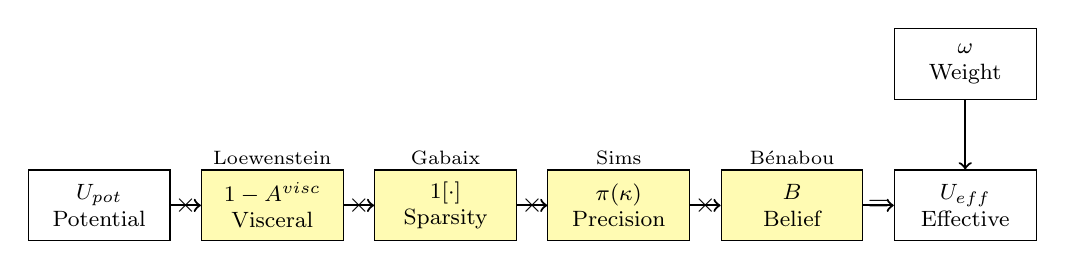
\begin{tikzpicture}[
    box/.style={rectangle, draw, minimum width=1.8cm, minimum height=0.9cm, align=center, font=\footnotesize},
    filter/.style={rectangle, draw, fill=yellow!30, minimum width=1.8cm, minimum height=0.9cm, align=center, font=\footnotesize},
    arrow/.style={->, thick},
    node distance=1.8cm
]

% Pipeline
\node[box] (upot) at (0,0) {$U_{pot}$\\Potential};
\node[filter] (visc) at (2.2,0) {$1-A^{visc}$\\Visceral};
\node[filter] (sparse) at (4.4,0) {$\mathbb{1}[\cdot]$\\Sparsity};
\node[filter] (ri) at (6.6,0) {$\pi(\kappa)$\\Precision};
\node[filter] (belief) at (8.8,0) {$B$\\Belief};
\node[box] (ueff) at (11,0) {$U_{eff}$\\Effective};

% Arrows
\draw[arrow] (upot) -- (visc);
\draw[arrow] (visc) -- (sparse);
\draw[arrow] (sparse) -- (ri);
\draw[arrow] (ri) -- (belief);
\draw[arrow] (belief) -- (ueff);

% Labels
\node[above=0.4cm, font=\scriptsize] at (visc) {Loewenstein};
\node[above=0.4cm, font=\scriptsize] at (sparse) {Gabaix};
\node[above=0.4cm, font=\scriptsize] at (ri) {Sims};
\node[above=0.4cm, font=\scriptsize] at (belief) {Bénabou};

% Multiplication signs
\node at (1.1,0) {$\times$};
\node at (3.3,0) {$\times$};
\node at (5.5,0) {$\times$};
\node at (7.7,0) {$\times$};
\node at (9.9,0) {$=$};

% Weight input
\node[box] (omega) at (11,1.8) {$\omega$\\Weight};
\draw[arrow] (omega) -- (ueff);

\end{tikzpicture}
\caption{The Awareness Pipeline: From Potential to Effective Utility}
\label{fig:awareness-pipeline}
\end{figure}

%------------------------------------------------------------------------------
\subsubsection{Summary: The Complete Specification}
\label{subsubsec:summary}
%------------------------------------------------------------------------------

\begin{tcolorbox}[colback=green!5!white, colframe=green!75!black, title=The Complete Awareness-Mediated Transformation]

\textbf{The Awareness Function:}
\begin{equation}
A_X = (1 - A^{visceral}) \times \mathbb{1}[stakes_X > m_X] \times \pi_X(\kappa) \times B_X(\hat{\theta}, signal, U_{IDN})
\end{equation}

\textbf{The Transformation:}
\begin{equation}
U^{eff}_X = U^{pot}_X \times A_X
\end{equation}

\textbf{The Effective Welfare:}
\begin{equation}
Q^{eff} = \sum_{j \in \{self, comm\}} \sum_{X \in \{INU, KNU, IDN\}} A^j_X \times \omega^j_X \times U^j_{pot,X}
\end{equation}

\end{tcolorbox}

This completes the formal specification of the Awareness function, integrating:
\begin{enumerate}
\item Visceral capture (Loewenstein)
\item Sparse attention (Gabaix)
\item Rational inattention (Sims)
\item Motivated beliefs (Bénabou \& Tirole)
\end{enumerate}

%------------------------------------------------------------------------------
\subsubsection{BEATRIX Module Reference}
\label{subsubsec:beatrix-ref}
%------------------------------------------------------------------------------

\begin{table}[htbp]
\centering
\caption{Section 11.08 BEATRIX References}
\label{tab:11-8-beatrix}
\renewcommand{\arraystretch}{1.3}
\begin{tabular}{@{}lll@{}}
\toprule
\textbf{Element} & \textbf{Module} & \textbf{Reference} \\
\midrule
Complete Awareness Function & AWX-A01 & Core Specification \\
Visceral Component & AWX-A10 & Loewenstein Override \\
Sparsity Component & AWX-A09 & Gabaix Threshold \\
Precision Component & AWX-A08 & Sims Allocation \\
Belief Filter Component & AWX-A04 & Bénabou Filter \\
Transformation Equation & AWX-A43 & Awareness-Multiplikation \\
Five Factors Model & BCM2\_05\_AWX\_7240\_01 & formal\_condition \\
\bottomrule
\end{tabular}
\end{table}

%%%%%%%%%%%%%%%%%%%%%%%%%%%%%%%%%%%%%%%%%%%%%%%%%%%%%%%%%%%%%%%%%%%%%%%%%%%%%%%
% END OF SECTION 11.08
%%%%%%%%%%%%%%%%%%%%%%%%%%%%%%%%%%%%%%%%%%%%%%%%%%%%%%%%%%%%%%%%%%%%%%%%%%%%%%%
